\newpage
{\bfseries МРНТИ 20.53.19}
\hfill {\bfseries \href{https://doi.org/10.58805/kazutb.v.3.24-340}{https://doi.org/10.58805/kazutb.v.3.24-340}}

\sectionwithauthors{Е.С.Кубегенов, А.Д. Кубегенова, А.Г. Жахиена, Г.Ш.Утешева, А.В. Нестеров}{ИНТЕЛЛЕКТУАЛДЫ ТЕХНОЛОГИЯЛАРДЫ ҚОЛДАНА ОТЫРЫП, ӘЛЕУМЕТТІК МАҢЫЗЫ
БАР АУРУЛАРДЫ ТАЛДАУ ЖӘНЕ ДЕРЕКТЕРДІ ӨҢДЕУ}
\begin{center}

{\bfseries \textsuperscript{1}Е.С.Кубегенов \envelope,
\textsuperscript{1}А.Д. Кубегенова, \textsuperscript{1}А.Г. Жахиена,
\textsuperscript{2}Г.Ш.Утешева, \textsuperscript{3}А.В. Нестеров}

\textsuperscript{1}Жәңгір хан атындағы Батыс Қазақстан
аграрлық-техникалық университеті, Орал, Қазақстан,

\textsuperscript{2}Батыс Қазақстан инновациялық-технологиялық
университеті, Орал, Қазақстан,

\textsuperscript{3}Г. В. Плеханов атындағы Ресей экономикалық
университеті, Мәскеу, Ресей
\end{center}
\envelope Корреспондент-автор: erlando78@mail.ru \vspace{0.5cm}

Қазіргі кезде интеллектуалды деректерді талдау көлемді деректер
жиынтығынан құнды ақпаратты алудың негізгі құралы болып табылады. Бұл
процесс жасырын үлгілерді, тенденцияларды және маңыз-ды үлгілерді
анықтауға мүмкіндік береді, бұл деректерді тереңірек түсінуге мүмкіндік
береді және негізделген шешімдер қабылдауға көмектеседі. Қазіргі
ақпараттық қоғамда деректерді өндіру медици-на, биология, экономика және
басқа да көптеген салаларда маңызды рөл атқарады. Оны қолдану адамдардың
өмір сүру сапасын жақсартуға, процестерді оңтайландыруға және әртүрлі
қызмет салала-рында тиімді стратегияларды жасауға ықпал етеді.

Бұл мақалада деректерді интеллектуалды талдау әдістерін пайдалана
отырып, Қазақстан Республи-касында туберкулезбен сырқаттанған жәнеде
қайтыс болғандардың динамикасы талданды. Республи-камыздың 2010-2022
жылдар аралығындағы деректерге ретроспективті талдау жүргізілді,
Statistica бағдарламалық жасақтама көмегімен және Data Mining әдістері
мен математикалық модельдер қолда-нылып, туберкулездің таралуына әсер
ететін негізгі факторлар анықталды.Статистикалық талдау жүргізуге,
байланыстар мен корреляцияларды анықтауға, сондай-ақ аурудың болашақ
дамуын бол-жауға мүмкіндік берді.

Сонымен қатар, зерттеу, ауруларды бақылау мен болжау мақсатында
интеграцияланған ақпараттық жүйелерді дамытудың маңыздылығы анықталды.
Бұл жүйелер деректерді жинау, өңдеу және сақтау процесін оңтайландырып,
эпидемиологиялық қауіптерге жедел жауап беруге мүмкіндік береді.
Мақа-лада туберкулез сияқты әлеуметтік маңызды ауруларды тиімді басқару
үшін интеллектуалды талдау әдістерін болашақта қолдану талқыланды.

{\bfseries Түйін сөздер:} болжау, интеллектуалды талдау, Data Mining,
статистикалық талдау, эпидемиоло-гия, корреляция.


\sectionheading{АНАЛИЗ СОЦИАЛЬНО ЗНАЧИМЫХ ЗАБОЛЕВАНИЙ И ОБРАБОТКА ДАННЫХ С
ИСПОЛЬЗОВАНИЕМ ИНТЕЛЛЕКТУАЛЬНЫХ ТЕХНОЛОГИЙ}
\begin{center}
{\bfseries \textsuperscript{1}Е.С. Кубегенов\textsuperscript{🖂},
\textsuperscript{1}А. Д. Кубегенова, \textsuperscript{1}А.Г.Жахиена,
\textsuperscript{2}Г.Ш. Утешева, \textsuperscript{3}А.В. Нестеров}

\textsuperscript{1}Западно-Казахстанский аграрно-технический университет
имени Жангир хана, Уральск, Казахстан,

\textsuperscript{2}Западно-Казахстанский инновационно-технологический
университет, Уральск, Казахстан.

\textsuperscript{3}Российский экономический университет им. Г.В.
Плеханова, Москва, Россия

e-mail:erlando78@mail.ru
\end{center}

В настоящее время интеллектуальный анализ данных является основным
инструментом для извле-чения ценной информации из объемных наборов
данных. Этот процесс позволяет выявлять скрытые закономерности,
тенденции и важные закономерности, обеспечивая более глубокое понимание
дан-ных и помогая принимать обоснованные решения. В современном
информационном обществе интел-лектуальный анализ данных играет важную
роль в медицине, биологии, экономике и многих других областях. Его
использование способствует улучшению качества жизни людей, оптимизации
процес-сов и разработке эффективных стратегий в различных сферах
деятельности.

В данной статье проанализирована динамика заболевших и умерших
туберкулезом в Республике Казахстан с использованием методов
интеллектуального анализа данных. Проведен ретроспективный анализ данных
республики за период 2010-2022 гг. с использованием программного
обеспечения Statistica, методов Data Mining и математических моделей,
выявлены основные факторы, влияющие на распространение туберкулеза.
Позволил провести статистический анализ, выявить связи и корре-ляции, а
также предсказать будущее развитие болезни.

Кроме того, была выявлена важность разработки интегрированных
информационных систем с целью исследований, мониторинга и
прогнозирования заболеваний. Эти системы позволяют оператив-но
реагировать на эпидемиологические угрозы, оптимизируя процесс сбора,
обработки и хранения данных. В статье обсуждалось использование методов
интеллектуального анализа в будущем для эффективного управления
социально значимыми заболеваниями, такими как туберкулез.

{\bfseries Ключевые слова:} прогнозирование, интеллектуальный анализ, Data
Mining, статистический ана-лиз, эпидемиология, корреляция.


\sectionheading{ANALYSIS OF SOCIALLY SIGNIFICANT DISEASES AND DATA PROCESSING
USING INTELLIGENT TECHNOLOGIES}
\begin{center}
{\bfseries \textsuperscript{1}E.S. Kubegenov\textsuperscript{🖂},
\textsuperscript{1}A.D. Kubegenova, \textsuperscript{1}A.G.Zhakhien,
G.Sh. Utesheva\textsuperscript{2}, A.V.Nesterov\textsuperscript{3}}

\textsuperscript{1}Zhangir Khan West Kazakhstan Agrarian Technical
University, Uralsk, Kazakhstan,

\textsuperscript{2}West Kazakhstan University of Innovation and
Technology, Uralsk, Kazakhstan,

\textsuperscript{3}Plekhanov Russian University of Economics, Moscow,
Russia

e-mail: erlando78@mail.ru
\end{center}

Currently, data mining is the main tool for extracting valuable
information from large datasets. This process allows you to identify
hidden patterns, trends, and important patterns, providing a deeper
understan-ding of the data and helping you make informed decisions. In
the modern information society, data mining plays an important role in
medicine, biology, economics and many other fields. Its use contributes
to improving the quality of people\textquotesingle s lives, optimizing
processes and developing effective strategies in various fields of
activity.

This article analyzes the dynamics of tuberculosis cases and deaths in
the Republic of Kazakhstan using data mining methods. A retrospective
analysis of the republic\textquotesingle s data for the period 2010-2022
was carried out using the Statistica software and using Data Mining
methods and mathematical models, the main factors influencing the spread
of tuberculosis were identified.It allowed to carry out statistical
analysis, identify connections and correlations, as well as predict the
future development of the disease.

In addition, the importance of developing integrated information systems
for the purpose of research, monitoring and forecasting of diseases was
identified. These systems allow you to quickly respond to
epidemiological threats, optimizing the process of data collection,
processing and storage. The article discussed the use of intellectual
analysis methods in the future for the effective management of socially
significant diseases such as tuberculosis.

{\bfseries Keywords:} forecasting, intelligent analysis, Data Mining,
statistical analysis, epidemiology, correlation.
\begin{multicols}{2}

{\bfseries Кіріспе.} Мақалада Қазақстан Республикасын-дағы жұқпалы
аурулардың мониторингі мен талдауы үшін медицинадағы деректерді
интеллектуалды талдау әдістері қарастырылған. Зерттеу нысаны ретінде
статистикалық шолудан 13 жылдағы (2010-2022) туберкулезбен
сырқаттанушылық көрсеткіштері алынды. Туберкулезден айыққан және қайтыс
болған науқастардың санын қамтитын ретроспективті талдау жүргізілді.

Data Mining технологиясын және StatisticaBase, StatisticaAdvanced, Data
Mining деректерді өндіру құралдары және SANN автоматтандырыл-ған
нейрондық желілерін қамтитын Statistica бағдарламалық пакетін пайдалана
отырып, үлкен деректерге бөлек талдау жүргізілді.

Коэффициентті есептеу және ретроспективті талдау арқылы корреляцияны
қолданудың практикалық маңыздылығы мен өзектілігі қазіргі ақпараттық
қоғамдағы мәліметтер мен оларды талдау нәтижелерінің маңыздылығымен
расталады.

Алынған нәтижелер туберкулез ауруының таралу динамикасын жақсы түсінуге
және оны алдын ала болжауға мүмкіндік береді.{[}1{]}

Қазақстан Республикасында туберкулез сияқты әлеуметтік маңызы бар
ауруларды талдаудың өзектілігі осы аурулардың халықтың денсаулығы мен
қоғамдық әл-ауқатына елеулі әсеріне байланысты.

Туберкулез ауруын бақылау, емдеу алдын алу жолдары жүргізілгенмен,
елдегі сырқаттанушы-лық пен өлім жітімнің басты себептерінің бірі болып
қала береді. Туберкулездің жоғары таралуы эпидемияны уақтылы анықтау
және алдын алу үшін тиімді бақылауды, талдауды және болжауды қажет
етеді, бұл жалпы денсаулық сақтау жүйесін жақсартуға ықпал етеді.

Зерттеу жұмысына қойылған мақсаттар:

1. 2010 жылдан 2022 жылға дейінгі кезеңде Қазақстан Республикасында
туберкулезбен сырқаттанушылық пен өлім-жітімге ретроспектив-ті талдау
жүргізу.

2. Деректерді өндіру әдістерін қолдана отырып, туберкулез ауруын алдағы
жылдарға таралу динамикасын болжау.

3. Туберкулездің таралуына әсер ететін негізгі факторларды анықтау.

4. Туберкулездің алдын алу және емдеу стратегияларын оңтайландыру
бойынша ұсыныстар әзірлеу.

Зерттеу жұмысsнда кездескен мәселелер:

1. Туберкулездің алдын алу мен емдеудің қазіргі стратегияларының
тиімділігінің жеткілік-сіздігі, бұл жоғары сырқаттанушылық пен өлімге
әкеледі.

2. Туберкулезді тиімдірек бақылау үшін оңтайландыруды қажет ететін
шектеулі Денсаулық сақтау ресурстары.

3. Туберкулездің жасырын түрлерінің болуы, бұл науқастарды уақтылы
анықтау мен емдеуді қиындатады.

4. Деректерді интеллектуалды өңдеудің заманауи әдістерін қамтитын
эпидемиологиялық жағдайды талдау мен болжауға кешенді көзқарастың
болмауы.

Зерттеу барысында күтілетін нәтижелерін атап өтсек:

1. 2010-2022 жылдар аралығындағы туберкулезбен сырқаттанушылық және
өлім-жітім динамикасын талдау, негізгі үрдістер мен өзгерістерді
анықтау.

2. Статистикалық талдау мен деректерді интеллектуалды өңдеу әдістерін
пайдалана отырып, туберкулездің таяу жылдарға таралуын болжау.

3. Эпидемиологиялық жағдайға әсер ететін негізгі факторларды және
олардың ауру мен өлімге әсерін анықтау.

4. Туберкулездің алдын алу және емдеу стратегияларын оңтайландыру үшін
ұсыныстар әзірлеу, бұл ауру мен өлімді азайтуға және денсаулық сақтау
ресурстарын тиімдірек пайдалануға ықпал етеді.

Бүгінгі таңда медицинадағы басқару мәселелерін шешу үшін математикалық
модельдеу әдістері, интеллектуалды тәсіл және интеллектуалды талдау жиі
қолданылады, бұл бір неше шешімдердін нұсқасын алуға, қабылданған
шешімдердің салдарын болжауға және оларды медициналық және әлеуметтік
тұрғыдан бағалауға көмектеседі.{[}2{]}

Эксперименттік мәліметтер квадратының статистикалық көрсеткіштерден
ауытқуы математикалық модельдегі параметрлерді сәйкестендірудің кері
есептерінің функциясының төмендеуін білдіреді. Статистикалық және
оңтайландыру алгоритмдерінің жиынтығын пайдалану параметрлерді
салыстырмалы 30\% дәлдікпен салыстыруға қол жеткізуге мүмкіндік береді.
Бұл нәтижелер Денсаулық сақтау ұйымдары үшін пайдалы болуы мүмкін, бұл
модельдеу деректерін тарихи деректермен салыстыру арқылы белгілі бір
аймақтағы жұқпалы аурулардың эпидемиясын болжауға мүмкіндік береді.

Жасанды интеллект-бұл аталған мәселелерді шешуге арналған, бірақ өзіндік
ерекшеліктерімен ерекшеленетін информатика саласы. Жұқпалы ауруларды
автоматты түрде анықтауға негізделген көптеген зерттеулер бар
туберкулез, АИТВ инфекциясы, COVID-19 және басқа вирустар симптомдарға
немесе әртүрлі белгілерге негізделген.

Компьютерлік және ақпараттық технологиялар-дың, сондай-ақ сақтау
технологияларының қарқынды дамуымен көптеген деректерді сақтауға болады
{[}3{]}.

Деректерді өндіру технологиясы көптеген деректерден әлеуетті құнды
білімді іздей және ала алады. Деректер базасының технологиясы-бұл
мәліметтер базасын басқаратын бағдарлама-лық жасақтама туралы ғылым.
Деректер базасынан алынған мәліметтер деректерді құрылымдау, жобалау
және қолдану әдістерін зерттеу арқылы талданады.{[}4{]}

Деректерді өндіру деректер үлгісін іздеу процесі ретінде анықталады,
яғни толық емес, анық емес, кездейсоқ деректердің үлкен санынан алынған
деректермен жұмыс істеу. {[}5{]}

Деректерді өндіру-бұл мәліметтер базасы мен жасанды интеллект
саласындағы өте белсенді зерттеу саласы.{[}6{]}

Деректерді компьютерлік интеллектуалды талдау технологиясын әзірлеуге
және қолдануға көп көңіл бөлу керек, өйткені деректерді өндіру
технологияларын қолдана отырып, біз тұрақты дамуға ықпал ететін тиімді
стратегияларды біріктіреміз.{[}7{]}

Эпидемиологияның математикалық моделінің мысалы (АИТВ-ның коинфекциясы
және туберкулез) математикалық модельдердің сәйкестігін зерттеуді
көрсетеді. {[}8{]}

Айнымалыларды математикалық анықталатын және біртекті ішкі жиындарға
көпөлшемді жіктеу көбінесе мәліметтер жиынтығына ресми статистикалық
талдау жасамас бұрын үлгіні танудың пайдалы алғашқы қадамы болып
табылады. Осындай әдістердің бірі, кластерлік талдау, жалпы
сипаттамалары мен деректер құрылымы бар объектілерді кластерлеудің
негізгі мақсатын көздейді. Мысалы, мұндай талдаудың мақсаттарының
бірі-жаңа деректерді оңай жіктеу үшін топқа жататындығын анықтау үшін
маңызды айнымалылар туралы түсінік алу; сонымен қатар, кластерленген
объектілермен байланысты айнымалыларды статистикалық талдауды жеңілдету
үшін белгілі бір жалпы сипаттамалары бар мәліметтер жиынтығын жасау
керек.{[}9{]}

Data Mining технологиясы бойынша эпидемиологиялық жағдайды талдау,
болжау және алдын ала анықтау жүргізу, өйткені қазіргі уақытта
Қазақстанда медициналық ақпаратты талдау үшін статистика әдістерін
қолдану жеткілікті кең таралмаған.

Туберкулезге қарсы қызмет жүйесіне деректерді компьютерлік өңдеуді
енгізе отырып, ауру туралы кешенді ақпаратты уақтылы жинақтау
эпидемиологиялық қадағалауды ақпараттық қамтамасыз ету деңгейін
арттыруға мүмкіндік береді.

Өлім саны бойынша туберкулез, АИТВ/ЖИТС және безгек сияқты аурулар әлі
де жетекші орында.

Туберкулез (туберкулез) (латын тілінен tuberculum -- туберкулез) --
денсаулығының нашарлауының негізгі себебі болып табылатын кең таралған
жұқпалы ауру, дүние жүзіндегі өлімнің 10 негізгі себебінің бірі.
Микобактерия тұқымдасының қышқылға төзімді бактериясы туберкулездің
қоздырғышы болып табылады. Жалпы, қазіргі уақытта микобактериялардың 74
түрі белгілі.

Жұқтырған адамның денесінде туберкулез қоздырғыштарының белгілі бір
тұрақты саны бар (жасырын күй), яғни олар негізінен лимфа түйіндерінде
локализацияланған және иммунитетпен тұрақты динамикалық тепе-теңдік
күйінде болады. Туберкулездің маңызды ерекшелігі-жасырын кезеңнің орташа
ұзақтығы өмір сүру ұзақтығымен салыстырылады, яғни адам бүкіл өмірін
жасырын жұқтырған кезде өткізе алады. Алайда, жаңадан жұқтырған
адамдардың шамалы бөлігі әлі де белсенді ауру жағдайына ауысады.{[}10{]}

Жыл сайын миллиондаған адамдар туберкулез-бен ауырады. Дүниежүзілік
денсаулық сақтау ұйымының (ДДҰ) 2012 жылғы жаһандық есебі туберкулез
эпидетін жан-жақты және өзекті бағалауды және жаһандық, аймақтық және
әлемдік деңгейдегі жауапты шаралардағы прогресті қамтиды.

Жаһандық есеп туберкулезбен сырқаттанушы-лық пен өлім-жітім үрдістерін,
көп дәріге төзімді туберкулезді, ТБ/АИТВ, туберкулездің алдын алу,
денсаулық сақтау қызметтерімен жалпы қамту, сондай-ақ қаржыландыру
жағдайларын анықтау және емдеу нәтижелері туралы деректерді қамтиды.
Онда 2018 жылы Біріккен Ұлттар Ұйымының туберкулез жөніндегі бас
Ассамблеясының жоғары деңгейдегі бірінші отырысында белгіленген
мақсаттарға, сондай-ақ ДДҰ-ның туберкулезге қарсы күрес Стратегиясының
мақсаттарына және тұрақты даму мақсаттарына (ТДМ) қол жеткізудегі
прогресс көрсетілген.{[}11{]}

Қазақстан Республикасы Дүниежүзілік денсаулық сақтау ұйымымен 2016-2020
жылдарға арналған ТБ МЛА ауыртпалығы жоғары елдер тізіміне енгізілген,
сондықтан осы жұқпалы аурумен күрес стратегиялық міндет болып қала
береді және ҚР ДСМ қызметіндегі басым бағыт болып табылады.

Қазақстан Республикасында туберкулез сияқты әлеуметтік маңызы бар
ауруларды талдаудың өзектілігі осы аурулардың халықтың денсаулығы мен
қоғамдық әл-ауқатына елеулі әсеріне байланысты. Туберкулез оны бақылау
мен емдеуге тырысқанына қарамастан, елдегі ауру мен өлімнің жетекші
себептерінің бірі болып қала береді. Туберкулездің таралуы эпидемияны
уақтылы анықтау және алдын алу үшін тиімді бақылауды, талдауды және
болжауды қажет етеді, бұл жалпы денсаулық сақтау жүйесін жақсартуға
ықпал етеді.

{\bfseries Материалдар мен әдістер.} С. Қайырбеков атындағы денсаулық
сақтауды дамытудың ұлттық ғылыми орталығынан «Қазақстан Республикасы
халқының денсаулығы және денсаулық сақтау ұйымдарының қызметі»
статистикалық жинақтан 2010 - 2022 жылдар аралығындағы туберкулезбен
ауырған, қайтыс болғандығы, бациллярлық есептен шығарылғандығы туралы
мәліметтер алынды. {[}12{]}

Қазақстан Республикасының 2010-2022 жылдар аралығында алынған деректерге
туберкулезбен сырқаттанған, бациллярлық есептен шығарылған және қайтыс
болған туралы мәліметтер бойынша (1-сурет) ретроспективті талдау
жүргізіліп, әрбір көрсеткіш бойынша өзгерістердің негізгі аспектілері
мен ықтимал себептерін қарастырдық.

\end{multicols}

\begin{figure}[H]
	\centering
	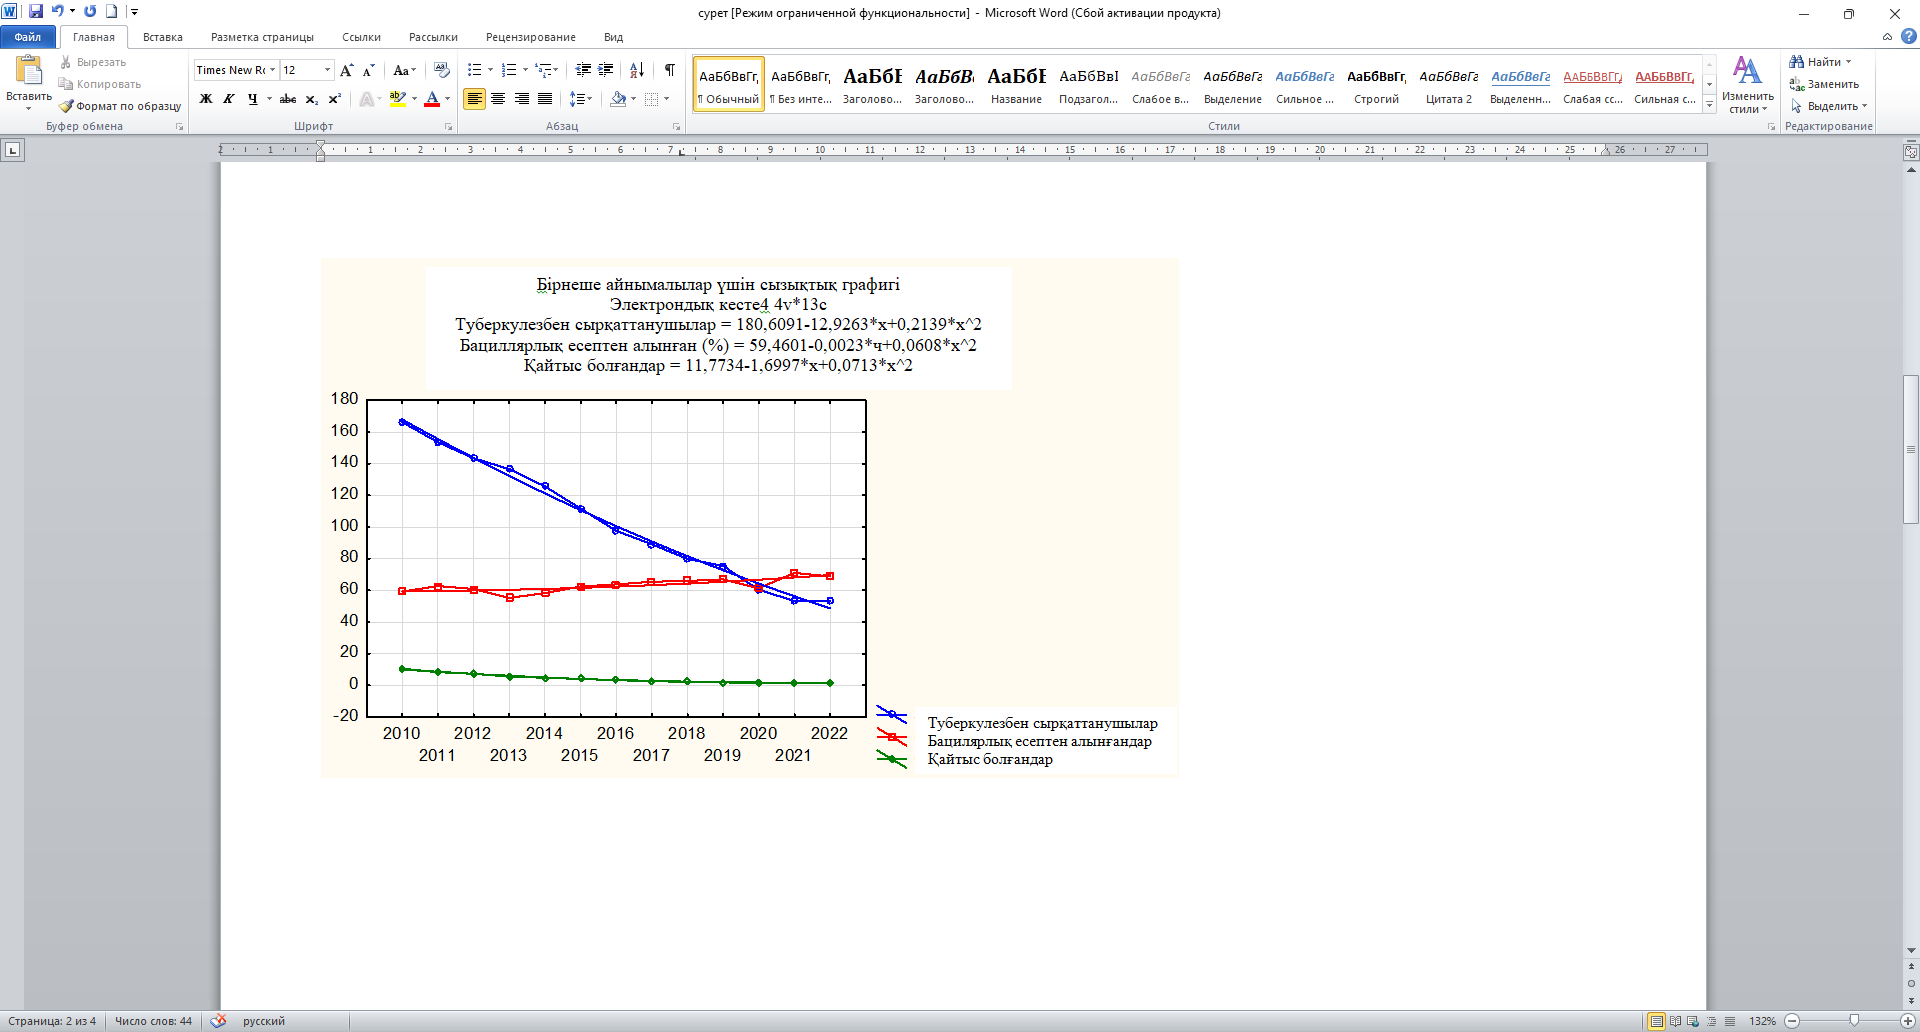
\includegraphics[width=0.7\textwidth]{assets/168}
	\caption*{1-сурет. Қазақстан Республикасының туберкулезбен
  сырқаттанушылығының 2010-2022 жылдар аралығындағы динамикасы}
\end{figure}


\begin{multicols}{2}

Сызықтық кестеде туберкулезбен ауыратын науқастар (көк сызық) аурушаңдық
2010 жылдан бері тұрақты түрде төмендеп келетіні байқалады. Бұған келесі
факторлар ықпал еткенін көруге болады:

\begin{enumerate}
\def\labelenumi{\arabic{enumi})}\setlength{\itemindent}{1cm}

\item
  соңғы жылдары елімізде туберкулезді ерте диагностикалау мен емдеу
  бағдарламаларын қолданып едәуір жақсарғаны. Химиотерапияның қысқа
  курстары сияқты жаңа емдеу әдістерін қолдану аурудың төмендеуіне әсер
  еткен болуы .
\item
  алдын алу шараларын күшейту, соның ішінде БЦЖ (Bacillus
  Calmette-Guérin) жаппай вакцинациялау және санитарлық-ағарту
  жұмыстарын жүргізу де аурудың төмендеуіне ықпал еткен болуы.
\item
  туберкулезбен күресуге бағытталған халықаралық көмек бағдарламалары
  ауруды төмендетуде маңызды рөл атқарғаны байқалады.
\end{enumerate}

Аурудың сызықтық кестесі (1 сурет) туберкулез (науқастардың, қайтыс
болғандардың саны және науқастарды бациллярлық есептен шығару) Қазақстан
Республикасының халқы бойынша 12 жылдық кезеңнің жиынтық деректері
ескеріле отырып 2010-2022 жылдар аралығында қарастырылды. Абсцисса осі
бойынша туберкулезбен ауыратын науқастарды зерттеу жылдары кейінге
қалдырылды, координаттар осі бойынша абсолютті сандар (халықтың 100 000
адамға шаққанда).

Бұл диаграмма 2010 - 2013 жылдар аралығында аурушаңдық бойынша тұрақты
үрдісті көрсетті. Нәтижесінде 2014 жылдан бастап аурушаңдықтың өсуі екі
есе нашарлағаның көріп тұрмыз.

Жалпы республика бойынша сырқаттанушылық-тың төмендеуі байқалғанымен,
туберкулез жаңа қасиеттерге ие болды. Науқастарда туберкулез
қоздырғышының дәріге төзбеушілігі және дәріге төзімділігі тұрақты
байқалады (1-сурет).

Жоғарыда көрсетілген кестелерді қарастырсақ, 2010 жылдан бастап
туберкулезбен сырқаттанушы-лық көрсеткіштерінің күрт төмендегенін бірден
байқауға болады, бірақ 2012 -- 2015 жылдар, 2016-2021 жылдар аралығында
қалыпты өрлеу мен құлдырау анықталуда. Сырқаттанушылық жағдайларының,
бұл күрт төмендеуі елдің туберкулезді инфекциялық бақылау шаралары,
емдеу, диагностика сапасы бойынша жаңа бағыттарға көшуімен байланысты
және туберкулездің алдын алу болып табылады.

Туберкулезді алдын алу, мәселесін шешу үшін эпидемияның болжамды ықтимал
ошағы үлкен рөл атқарады. Сондықтан болжау жүйесін құру немесе
математикалық модельдерді қолдану негіздері бұрыннан қолданғанмен
интеллектуалды жүйелерді пайдалану маңызды болып келеді. Белгілі бір
аймақты нақты және дәл сипаттайтын модельді таңдау жасау.{[}13{]}
\end{multicols}
\begin{table}[H]
  \caption*{Кесте 1. Сипаттамалық статистика нәтижелері}
  \resizebox{\textwidth}{!}{ % Adjust the width as needed
    \begin{tabular}{|c|ccccc|}
      \hline
      \multicolumn{1}{|l|}{\multirow{2}{*}{\textbf{Айнымалы}}} &
      \multicolumn{5}{l|}{\textbf{Сипаттамалық статистика}}\\ \cline{2-6} 
      \multicolumn{1}{|l|}{} &
      \multicolumn{1}{l|}{\textbf{жарамды N}} &
      \multicolumn{1}{l|}{\textbf{Орташа}} &
      \multicolumn{1}{l|}{\textbf{Минимум}} &
      \multicolumn{1}{l|}{\textbf{Максимум}} &
      \multicolumn{1}{l|}{\textbf{Стандартты анықтама}} \\ \hline
      Туберкулезбен сырқаттанушы &
      \multicolumn{1}{c|}{13} &
      \multicolumn{1}{c|}{103,6000} &
      \multicolumn{1}{c|}{53,30000} &
      \multicolumn{1}{c|}{166,3000} &
      38,90180 \\ \hline
      Бациллярлық есептен алынды (\%) &
      \multicolumn{1}{c|}{13} &
      \multicolumn{1}{c|}{63,2769} &
      \multicolumn{1}{c|}{55,30000} &
      \multicolumn{1}{c|}{71,1000} &
      4,40854 \\ \hline
      Қайтыс болған &
      \multicolumn{1}{c|}{13} &
      \multicolumn{1}{c|}{4,3692} &
      \multicolumn{1}{c|}{1,40000} &
      \multicolumn{1}{c|}{10,6000} &
      2,89349 \\ \hline
    \end{tabular}
  }
\end{table}


\begin{multicols}{2}

2010-2022 жылдар аралығының кезеңінде туберкулезбен сырқаттанушылықтың
сипаттамалық статистикасын талдау негізінде мынадай тұжырымдар жасауға
болады:(2-сурет)

\begin{itemize}
  \setlength{\itemindent}{1cm}
\item
  туберкулез ауруының орташа жиілігі 103,6000 жағдайды құрайды (халықтың
  100 000 адамға шаққанда)
\item
  ең төменгі мәні туберкулезбен сырқаттану-шылық 53,30000(халықтың 100
  000 адамға шаққанда), туберкулезбен сырқаттанушылықтың ең жоғары
  деңгейі 166,30 000(халықтың 100 000 адамға шаққанда) құрайды - бұл
  зерттеу кезеңінде туберкулезбен сырқаттанушылықтың айтарлықтай
  өзгергенің көрсетеді;
\item
  аурудың стандартты ауытқуы 38,90180 бұл орташа мәнге қатысты мәндердің
  таралуын көрсетеді. Стандартты ауытқудың үлкен мәні деректердің
  айтарлықтай өзгергіштігін көрсетеді;
\item
  бациллярлық есептен шығару (яғни туберкулезден айыққан немесе қайтыс
  болған науқастардың саны) орташа мәні 63,2769, ең төменгі мәні 5,30000
  және ең жоғары мәні 71,1000 құрайды. Бұл пациенттердің көпшілігі
  туберкулезден сәтті емделетінін көрсетеді, бірақ өлім жағдайы да бар;
\item
  Туберкулезден болатын өлім-жітімнің орташа мәні 4,3692, ең төменгі
  мәні 1,40000 және ең жоғары мәні 10,6000 -- бұл туберкулезден болатын
  өлім-жітімнің бар екендігін көрсетеді.
\end{itemize}

Негізінде сипаттамалық статистиканың нәтижелері туберкулезбен
сырқаттанушылықтың өзгергіштік деңгейі жоғары екенін көрсетеді,
сондай-ақ осы аурудан сырқаттанушылық пен өлім-жітімді төмендету
шараларын қабылдау қажеттігін көрсетеді.


\end{multicols}

\begin{figure}[H]
	\centering
	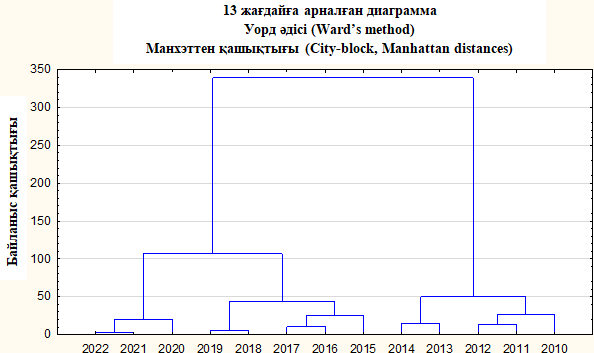
\includegraphics[width=0.7\textwidth]{assets/169}
	\caption*{\bfseries 2-сурет. Қазақстан Республикасының 2010-2022 жылдар кезеңінде
  туберкулезбен сырқаттанушылық жөніндегі Дендрограмма}
\end{figure}


\begin{multicols}{2}

Деректерді өңдеуге, визуалиациялауға және иерархиялық кластерлеуді
орындау үшін жиі қолданылатын бағдарламалардын бірі Statistica болып
келеді. Осы бағдарлама арқылы деректерді ұқсастығына немесе
айырмашылығына қарай топтастыру үшін Уорд әдісі (Ward's method) және
Манхэттен қашықтығы (City-block, Manhattan distances) сияқты әртүрлі
кластерлеу әдістерін қолданылды. Статистикадағы Дендрограмма
зерттеушілерге күрделі уақыт қатарларын визуализациялауға және талдауға
және анықталған деректер негізінде ақпараттандырыл-ған шешімдер
қабылдауға мүмкіндік береді.

Дендрограммада (Сурет 2) көлденең осьта 2010 және 2022 жылдар
аралығындаағы кезеңінде туберкулезбен сырқаттанғаны көрсетілген, ал
тігінен -- бірігу қашықтығын білдіреді. Бүкіл кезең екі үлкен кластерге
бөлінеді: 2010-2014 жылдар және 2015-2022 жылдар. Бұл екі кезеңдегі
туберкулезбен сырқаттанушылық туралы мәліметтер бір-бірінен айтарлықтай
ерекшеленетінін көрсетіп тұр.

1 кластерде 2021-2022, 2019-2020, және 2015-2018 кіші топтарға бөлінген

Соңғы 2021 және 2022 жылдар жеке кіші топты құрайды, бұл осы кезеңдегі
аурудың ерекше динамикасын көрсетіп тұрғанын көреміз, мүмкін соңғы
жылдары қабылданған шаралармен немесе есептіліктің өзгеруімен
байланысты. 2019 және 2020 жылдар да бөлек топтастырылған, бұл COVID-19
пандемиясының осы кезеңдегі туберкулез статистикасына әсерін көрсетуі
деп білеміз

2 кластер 2010-2014 жылдар аралығы көрсеткіштері тұрақтылықты көрсетіп
тұр.

Дендрограмма туберкулезбен ауыру динамика-сында, әсіресе 2014-2015 жылдар
аралығында айтарлықтай өзгерістердің болуын болжайды, бұл емдеу
стратегияларының, Денсаулық сақтау саясатының немесе басқа сыртқы
факторлардың өзгеруіне байланысты болуы мүмкін.Соңғы жылдардағы кіші
топтар (2019-2022) талдау үшін ерекше назар аударуды қажет етеді,
өйткені олар ауру динамикасындағы жаңа бағытты көрсете алады.

Бұл деректер белгілі бір кезеңде туберкулез ауруының мұндай өзгеруіне не
себеп болуы мүмкін екенін жақсы түсіну үшін қосымша талдау үшін қажет
етеді.

Statistica бағдарламасында жасалған дендро-грамма нақты математикалық
модельдерге негізделген иерархиялық деректер кластерінің визуализациясы
болып табылады. Бұл дендрограмма кластерлерді біріктіру үшін Уорд әдісін
және деректер арасындағы қашықтықты есептеу үшін Манхэттен қашықтығын
(City-block, Manhattan distances) пайдаланады.{[}14{]}

Оларды бөлек талдап көретін болсақ:

Уорд әдісінің (Ward's method) (формула2) мақсаты кластерлерді
біріктірудің әрбір қадамында жалпы кластерішілік дисперсияның ұлғаюын
азайту.
\end{multicols}

\begin{equation}
  \Delta E - \sum_{i=1}^{n_1} (x_i - \overline{x_1})^2 + \sum_{j=1}^n (y_j - \overline{y_2})^2 - \sum_{k=1}^{n_1 +n_2} (z_k - \overline{z})^2
\end{equation}

Бұндағы:

$n_1$ және $n_2$- 1 және 2 кластерлердегі элементтер
саны.

$x_i$ және $y_i$- 1 және 2 кластер элементтері

$\overline{x_1}$ және $\overline{y_2}$- 1 және 2 кластерлер бойынша орташа
мәндер.

$z_k$ - біріктірілген кластер элементтері.

$\overline{z}$ - біріктірілген кластердің орташа
мәні.

Уорд әдісінің (Ward's method) мақсаты $\triangle E$азайту болып келеді бұл екі
кластерді біріктіру кезінде кластер ішіндегі дисперсияның өзгеруін
білдіреді..

Манхэттен қашықтығы (City-block, Manhattan distances) (формула 2)әдістің
мақсаты: жылдар арасын-дағы ұқсастықтарды есептеу үшін қолданылатын көп
өлшемді кеңістіктегі екі нүкте арасындағы қашықтықты анықтау болып
табылады.

\begin{equation}
  d(i,j) = - \sum_{k-1}^n |x_{ik} - x_{jk}|
\end{equation}

Бұндағы:

$d(i,j)$ - Манхэттеннің нүктелер арасындағы
қашықтығы $i$ және $j$

$x_{ik}$ және $x_{jk}$ - $i$ және $j$ нүкте координаттарының $k$өлшемі

$n$- өлшеу саны

Манхэттен қашықтығы (City-block, Manhattan distances)әр өлшемдегі
нүктелердің координаттары арасындағы жалпы абсолютті айырмашылықты
өлшейді.

Дендрограмманың жалпы моделі:

\begin{enumerate}
\def\labelenumi{\arabic{enumi}.}\setlength{\itemindent}{1cm}
\item
  Кластерлеудің әр кезеңінде екі кластер таңдалады, олардың арасындағы
  қашықтық Манхэттен метрикасы бойынша минималды. Содан кейін бұл
  кластерлер біріктіріліп, процедура барлық нысан-дар бір кластерде
  болғанша қайталанады.
\item
  Біріктіру процесі Уорд әдісін (Ward's method) қолдану арқылы қол
  жеткізілетін кластерішілік дисперсияның ұлғаюын азайту үшін жүреді.
\end{enumerate}

Осылайша, дендрограмма кластер ішіндегі дисперсияны азайту және
Манхэттен метрикасы бойын-ша қашықтықты есептеу негізінде кластерлерді
дәйекті біріктіру процесінің графикалық көрінісі болып табылады.
\begin{multicols}{2}

{\bfseries Нәтижелер мен талқылау.} Бұл зерттеу туберкулез сияқты ауруларды
бақылау және талдау саласына маңызды үлес қосады. Деректер мен
математикалық модельдерді қолдану аурудың динамикасын түсінуге ғана
емес, сонымен қатар аурудың таралуына әсер ететін факторларды анықтауға
мүмкіндік береді. Деректерді жинауды, өңдеуді және талдауды
автоматтандыруға қабілетті интеграцияланған ақпараттық жүйелерді дамыту
ауруларды тиімді бақылау мен бақылаудың негізгі элементі болып табылады.
Зерттеу қоғамдық денсаулық пен халықтың өмір сүру сапасын жақсарту үшін
деректерді өндіру саласындағы жұмыстарды жалғастырудың маңыздылығын
көрсетеді.

Туберкулез сияқты әлеуметтік маңызы бар аурулардың мониторингінде
деректерді интеллектуалды талдауды қолдану оның болашақ даму үшін
маңыздылығы мен әлеуетін көрсетеді. Data Mining математикалық модельдері
мен әдістеріне негізделген зерттеу 2010-2022 жылдар аралығында Қазақстан
Республикасында туберкулезбен сырқаттанушылықтың динамикасын терең
түсіну мүмкіндіктерін көрсетеді, бұл мақсатты профилактикалық және емдік
іс-шараларды әзірлеуге ықпал ететін үрдістер мен ықпал ететін
факторларды анықтайды. Деректерді интеллектуалды талдау
сырқаттанушылықтың динамикасын көзбен көріп, болжап қана қоймай, сонымен
қатар халықтың көші-қоны, өмір сүру деңгейі, медициналық қызмет көрсету
деңгейі, медициналық қызмет көрсету шығындары сияқты сырқаттанушылық пен
басқа да әлеуметтік маңызы бар факторлар арасында байланыс орнатуға,
түрлі аймақтар бойынша талдау жүргізуге мүмкіндік береді.

Демек, ауру деректерін автоматтандырылған бақылау мен талдауға арналған
интеграцияланған ақпараттық жүйені әзірлеу және енгізу қажеттілігі
туындайды.

Мұндай жүйе талдау және болжау құралдарын ұсына отырып, деректерді
жинауды, өңдеуді және сақтауды жақсартуға уәде береді, бұл ауру деңгейін
тиімдірек төмендетуге және эпидемиологиялық қауіптерге жауап беруге
мүмкіндік береді.{[}15{]}

Алдын ала талдау жоспарланған ақпараттық жүйе мынадай блоктардан тұруы
тиіс екенін көрсетті: деректерді қабылдау, тазарту, трансформациялау;
деректер қоймасы; деректерді статистикалық талдау блогы; деректерді
интеллектуалды талдау блогы; болжамдарды қалыптастыру блогы; есептерді
қалыптастыру блогы; деректерді визуализациялау блогы.

Зерттеудің маңыздылығы: деректерді жинау, өңдеу және талдау процестерін
автоматтандырудың қоғамдық денсаулық сақтауды жақсартудағы маңыздылығын
айқын көрсетеді. Интеграцияланған ақпараттық жүйелердің көмегімен үлкен
көлемдегі деректерді тиімді басқару және талдау аурудың таралу
динамикасын жақсы түсінуге мүмкіндік береді. Мұндай жүйелер нақты
уақыттағы эпидемияларды анықтау және алдын алу үшін аса қажет.

Зерттеу нәтижесінде 2010-2022 жылдар аралығында туберкулездің таралуы
бойынша деректерге негізделген болжау жасалды. Data Mining және
статистикалық әдістері туберкулезбен сырқаттанушылықтың болашақ
динамикасын анықтауға және соған сәйкес алдын алу шараларын жоспарлауға
мүмкіндік береді. Мысалы, 2020-2022 жылдардағы дендрограмма мен
графиктерде көрінген ауру деңгейінің өзгерістері емдеу және алдын алу
шараларының тиімділігін көрсетті.

Алынған нәтижелер 2010-2022 жылдардағы туберкулезбен сырқаттанушылық пен
өлім-жітім динамикасында айтарлықтай төмендеу байқалғанын көрсетеді.
Сырқаттанушылықтың төмендеуі денсаулық сақтау жүйесінде жүргізілген
алдын алу және емдеу шараларының тиімділігін көрсетсе, өлім-жітімнің
төмендеуі тиімді емдеу шараларының нәтижесі болуы мүмкін.

Деректерді интеллектуалды өңдеу арқылы аурудың таралуына әсер ететін
негізгі факторлар анықталды. Бұл факторлар туберкулездің аймақтық
ерекшеліктеріне, халықтың әлеуметтік-экономикалық жағдайына және
медициналық ресурстардың қолжетімділігіне байланысты болуы
мүмкін.Туберкулездің таралуын болжау және негізгі факторларды анықтау
болашақта мақсатты профилактикалық іс-шараларды ұйымдастыруға ықпал
етеді. Бұл алынған мәліметтерді емдеу стратегияларын жетілдіру үшін
қолдануға болады.

Зерттеу барысында жасалған математикалық модельдер мен статистикалық
әдістер Қазақстан Республикасында туберкулездің өршігу динамикасын
тереңірек түсінуге мүмкіндік берді. Деректерді интеллектуалды өңдеу
нәтижесінде алынған нәтижелер туберкулездің өршігуне әсер ететін негізгі
факторларды анықтап қана қоймай, оның болашақта қалай жетілуінің
болжауға көмектеседі. Бұл ауруды бақылау және алдын алу шараларын
жетілдіру үшін маңызды ақпарат болып табылады. Туберкулездің таралуын
болжау бойынша алынған нәтижелер денсаулық сақтау жүйесіне орасан зор
үлес қосып, оның қоғамдық денсаулыққа әсерін азайтуға мүмкіндік береді.

{\bfseries Қорытынды.} Бұл зерттеу Қазақстан Республикасында 2010-2022
жылдар аралығында-ғы туберкулезбен сырқаттанушылықтың динамикасын талдау
арқылы әлеуметтік маңызы бар ауруларды бақылаудың заманауи әдістерінің
маңыздылығын көрсетіп, деректерді интеллектуалды өңдеу мен математикалық
модельдеу әдістерін қолдану барысында туберкулез аурудын таралуын, оның
өлім-жітім көрсеткіштерін және емдеу нәтижелерін болжауға мүмкіндік
берді.

Зерттеу барысында туберкулездің өршігу динамикасын талдау үшін деректер
арасындағы айырмашылықтарды анықтау үшін, Манхэттен
қашықтығы(City-block, Manhattan distances) және Уорд
(Ward\textquotesingle s Method) кластерлеу әдістері қолданылып
объектілер арасындағы айырмашылықтарды бірқатар факторлар бойынша
өлшеуге мүмкіндік берді. Нәтижесінде, туберкулезбен сырқаттанушылықтың
әртүрлі жылдардағы деңгейлерінің ұқсастығы мен айырмашылықтары
анықталды.

Ал, Уорд әдісі (Ward\textquotesingle s Method) кластерлеуді жүргізу
барысында топтар арасындағы дисперсияны минимизациялау принципіне
негізделіп, деректерді ұқсас топтарға біріктіру арқылы жылдар арасындағы
корреляцияны айқындап, туберкулездің өршігу үрдістерін көрсететін
иерархиялық құрылымдарды жасауға мүмкіндік берді.

Нәтижесінде, белгілі бір жылдар арасындағы сырқаттанушылықтың өзара
ұқсастықтары анықталып, дендрограммада құрылды.

Уорд әдісі (Ward\textquotesingle s Method) мен Манхэттен қашықтығын
(City-block, Manhattan distances) қолдану эпидемиологиялық деректерді
топтасты-руда және оларды талдауда тиімді әдіс ретінде маңызды рөл
атқаратыны, туберкулез ауруының өршігуі бойынша динамикалық өзгерістерді
айқындауға, әртүрлі жылдардағы сырқаттанушылардың көрсеткіштерінің ұқсас
кезеңдерін анықтауға және оларды болашақта болжау үшін қолдануға
болатыны дәлелденді деуге болады.

Алынған нәтижелер денсаулық сақтау жүйесіне стратегиялық шешімдер
қабылдауда нақты негізі болып, эпидемиологиялық жағдайды тиімді
басқаруға ықпал етеді.

Бұл әдістер эпидемияларды уақтылы анықтау, тиімді бақылау және олардың
әсерін азайту үшін денсаулық сақтау жүйесін оңтайландыруға көмектеседі.

Қорытындылай келе, туберкулездің таралуын болжау мақсатында заманауи
әдістерді қолдану Қазақстандағы қоғамдық денсаулықты жақсарту және осы
аурумен күрестің тиімділігін арттыру үшін маңызды қадам болып табылады.

\end{multicols}


\begin{center}
  {\bfseries Әдебиеттер}
  \end{center}

\begin{noparindent}

\begin{enumerate}
\def\labelenumi{\arabic{enumi}.}
\item
  Кубегенова А., Искаков К., Кубегенов Е., Криворотько О. Мониторинг и
  моделирование эпидемио-логической ситуации с помощью интеллектуального
  анализа данных // Известия НАН РК. Серия физико-математическая. -№
  4(2022). --С. 43-55. DOI: https://doi.org/10.32014/2022.2518-1726.155
\item
  Юнкеров В.И. Математико-статистическая обработка данных медицинских
  исследований / В.И. Юнкеров, С.Г. Григорьев. -- СПб.: ВМедА, 2002. --
  266 с. ISBN 5-94277-011-5
\item
  Барсегян А. А. С. Куприянов, И. И. Холод, М. Д. Тесс, С.И. Елизаров
  Анализ данных и процессов: учеб. пособие /-- 3-е изд., перераб. и доп.
  -- СПб.: БХВ-Петербург, 2009-- 512 с. ISBN 978-5-9775-0368-6
\item
  Xinyi Wang. The Role of Data Mining Technology in Advertising
  Marketing // J. Phys.: Conf. Ser. -2021. --Vol. 1744(4). DOI:
  10.1088/1742-6596/1744/4/042202
\item
  Jianguo Liu \& Sheng Zhou~Application Research of Data Mining
  Technology in Personal Privacy Protection and Material Data Analysis
  // Integrated Ferroelectrics. -2021. --Vol.216. --P. ~29-42.
 \\DOI:~10.1080/10584587.2021.1911255
\item
  He, Wu, Gongjun Yan, and Li Da Xu. Developing vehicular data cloud
  services in the IoT environment //IEEE
  transactionsonindustrialinformatics. -2014. --Vol. 10(2). -P.
  1587-1595. DOI:10.1109/TII.2014.\\2299233
\item
  Peña-Ayala, Alejandro Educational data mining: A survey and a data
  mining-based analysis of recent works // Expertsystemswith
  applications. -2014. --Vol.41(4). --Vol.1432-1462.
  DOI:10.1016/j.eswa.2013.\\08.042
\item
  Zhenhua HUANG, Zhenyu WANG,~Li JIANG,~Rui ZHANG,~Chang LEI,~Xingwei
  LIU,~Xiaohui XIE Analysis of COVID-19 spread characteristics and
  infection numbers based on large-scale structured case data //
  Scientia Sinica Informationis. -2020--Vol. 50(12).
  DOI:10.1360/SSI-2020-0029
\item
  Cross C. L. Statistical and methodological considerations when using
  cluster analysis in neuropsychological research //Cluster analysis in
  neuropsychological research: Recent applications. -- New York, NY :
  Springer New York, 2013. --Vol. 25(5). -- P. 13-35.
  DOI:10.1007/978-1-4614-6744-1\_2
\item
  Мельниченко О.А., Романюха А.А. Модель эпидемиологии туберкулеза.
  Анализ данных и оценка параметров // Математическое моделирование. --
  2008. -- №8. -- С.107-128.\\URL:
  https://www.mathnet.ru/links/8eaf4b16128064394600eb860acd44ba/mm2678.pdf
\item
  Генеральная Ассамблея. Организация Объединенных Наций.
  \\https://documents.un.org/doc/undoc/gen/n23/306/93/pdf/n2330693.pdf
\item
  Национальный научный центр развития здравоохранения имени
  С.Каирбекова. Статистические сборники «Здоровье населения~ Республики
  Казахстан и деятельность организаций~ здравоохранения».~ \\https://nrchd.kz/index.php/ru/?option=com\_content\&view=article\&id=973

\item
  Kubegenova, A.D., Zhakhiena, A.G., Baigubenova, S.K., Utyasheva, G.S.,
  Omarov, A.N. Clustering and data mining on the example of hiv-infected
  people data
  \emph{//~}Journal of Theoretical and Applied Information
  Technology\emph{.} -2022. --Vol.100~(13). -P.~5010-5018.URL:
  https://jatit.org/volumes/Vol100\\No13/30Vol100No13.pdf
\item
  King R. S. Cluster analysis and data mining: An introduction. --
  Mercury Learning and Information, 2015. ISBN 978-1-938549-38-0
\item
  Kubegenova A.D.,KamalovaG.A., Kubegenov, E.S., Gumarova, Z.M.,
  Zhazykbaeva, G.M. Using Data Mining Technology in Monitoring and
  Modeling the Epidemiological Situation of the Human Immuno\\deficiency
  Virus in Kazakhstan // Information Technologies and Intelligent
  Decision-Making Systems. -2022. -Vol 1703. --P. 57-65.
  DOI:10.1007/978-3-031-21340-3\_6
\end{enumerate}

\end{noparindent}

\begin{center}
  {\bfseries References}
  \end{center}

\begin{noparindent}

1. Kubegenova A., Iskakov K., Kubegenov E., Krivorot\textquotesingle ko
O. Monitoring i modelirovanie jepidemiologiches\\koj situacii s
pomoshh\textquotesingle ju intellektual\textquotesingle nogo analiza
dannyh // Izvestija NAN RK. Serija fiziko-matematiches\\kaja. -№ 4(2022).
--S. 43-55. DOI: https://doi.org/10.32014/2022.2518-1726.155 {[}in
Russian{]}

2. Junkerov V.I. Matematiko-statisticheskaja obrabotka dannyh
medicinskih issledovanij / V.I. Junkerov, S.G.
Grigor\textquotesingle ev. -- SPb.: VMedA, 2002. -- 266 s. ISBN
5-94277-011-5 {[}in Russian{]}

3. Barsegjan A. A. S. Kuprijanov, I. I. Holod, M. D. Tess, S.I. Elizarov
Analiz dannyh i processov: ucheb. posobie /-- 3-e izd., pererab. i dop.
-- SPb.: BHV-Peterburg, 2009-- 512 s. ISBN 978-5-9775-0368-6 {[}in
Russian{]}

4. Xinyi Wang. The Role of Data Mining Technology in Advertising
Marketing // J. Phys.: Conf. Ser. -2021. --Vol. 1744(4). DOI:
10.1088/1742-6596/1744/4/042202

5. Jianguo Liu \& Sheng Zhou Application Research of Data Mining
Technology in Personal Privacy Protection and Material Data Analysis //
Integrated Ferroelectrics. -2021. --Vol.216. --P. 29-42. DOI:
10.1080/10584587.2021.1911255

6. He, Wu, Gongjun Yan, and Li Da Xu. Developing vehicular data cloud
services in the IoT environment // IEEE
transactionsonindustrialinformatics. -2014. --Vol. 10(2). -P. 1587-1595.
DOI:10.1109/TII.2014.\\2299233

7. Peña-Ayala, Alejandro Educational data mining: A survey and a data
mining-based analysis of recent works // Expertsystemswith applications.
-2014. --Vol.41(4). --Vol.1432-1462. DOI:10.1016/j.eswa.2013.\\08.042

8. Zhenhua HUANG, Zhenyu WANG, Li JIANG, Rui ZHANG, Chang LEI, Xingwei
LIU, Xiaohui XIE Analysis of COVID-19 spread characteristics and
infection numbers based on large-scale structured case data // Scientia
Sinica Informationis. -2020--Vol. 50(12). DOI:10.1360/SSI-2020-0029

9. Cross C. L. Statistical and methodological considerations when using
cluster analysis in neuropsychological research //Cluster analysis in
neuropsychological research: Recent applications. -- New York, NY :
Springer New York, 2013. --Vol. 25(5). -- P. 13-35.
DOI:10.1007/978-1-4614-6744-1\_2

10. Mel\textquotesingle nichenko O.A., Romanjuha A.A.
Model\textquotesingle{} jepidemiologii tuberkuleza. Analiz dannyh i
ocenka parametrov // Matematicheskoe modelirovanie. -- 2008. -- №8. --
S.107-128. \\URL:
https://www.mathnet.ru/links/8eaf4b16128064394600eb860acd44ba/mm2678.pdf
{[}in Russian{]}

11. General\textquotesingle naja Assambleja. Organizacija Ob\#edinennyh
Nacij.
\\https://documents.un.org/doc/undoc/gen/n23/306/93/pdf/n2330693.pdf {[}in
Russian{]}

12. Nacional\textquotesingle nyj nauchnyj centr razvitija
zdravoohranenija imeni S.Kairbekova. Statisticheskie sborniki
«Zdorov\textquotesingle e naselenija Respubliki Kazahstan i
dejatel\textquotesingle nost\textquotesingle{} organizacij
zdravoohranenija».
URL:
https://nrchd.kz/index.php/ru/?option=com\_content\&view=article\&id=973
{[}in Russian{]}

13. Kubegenova, A.D., Zhakhiena, A.G., Baigubenova, S.K., Utyasheva,
G.S., Omarov, A.N. Clustering and data mining on the example of
hiv-infected people data

// Journal of Theoretical and Applied Information Technology. -2022.
--Vol.100 (13). -P. 5010-5018.\\ URL:
https://jatit.org/volumes/Vol100No13/30Vol100No13.pdf

14. King R. S. Cluster analysis and data mining: An introduction. --
Mercury Learning and Information, 2015. ISBN 978-1-938549-38-0

15. Kubegenova A.D.,KamalovaG.A., Kubegenov, E.S., Gumarova, Z.M.,
Zhazykbaeva, G.M. Using Data Mining Technology in Monitoring and
Modeling the Epidemiological Situation of the Human Immuno\\deficiency
Virus in Kazakhstan // Information Technologies and Intelligent
Decision-Making Systems. -2022. -Vol 1703. --P. 57-65.
DOI:10.1007/978-3-031-21340-3\_6
\end{noparindent}


\emph{{\bfseries Information about the authors}}
\begin{noparindent}

Kubegenov E.S. -- Senior Lecturer, Zhangir Khan West Kazakhstan Agrarian
Technical University, Uralsk, Kazakhstan, e-mail: erlando78@mail.ru;

Kubegenova A.D. -- Senior Lecturer, Master\textquotesingle s degree,
Zhangir Khan West Kazakhstan Agrarian Technical University, Uralsk,
Kazakhstan, e-mail: aigul-03@mail.ru;

Zhakhiena A.G. - Senior Lecturer, Master\textquotesingle s degree,
Zhangir Khan West Kazakhstan Agrarian Technical University, Uralsk,
Kazakhstan, e-mail: aizatmail@mail.ru;

Utesheva G.Sh.- Senior Lecturer, Master\textquotesingle s degree, West
Kazakhstan University of Innovation and \\Technology, Uralsk, Kazakhstan,
e-mail:utesheva.gulnara@mail.ru;

Nesterov A.V.- Ph.D., Professor Plekhanov Russian University of
Economics, Moscow, Russia, e-mail: nesterov.av@rea.ru
\end{noparindent}

\emph{{\bfseries Сведения об авторах}}
\begin{noparindent}

Кубегенов Е.С. -- старший преподователь,Западно-Казахстанский
аграрно-технический университет имени Жангир хана, Уральск,
Казахстан,e-mail:erlando78@mail.ru;

Кубегенова А. Д. -- старший преподаватель, магистр Западно-Казахстанский
аграрно-технический университет имени Жангир хана, Уральск,
e-mail:aigul-03@mail.ru;

Жахиена А.Г.- старший преподаватель,магистр, Западно-Казахстанский
аграрно-технический универ-ситет имени Жангир хана, Уральск, Казахстан,
e-mail: aizatmail@mail.ru;

Утешева Г.Ш.-старший преподаватель, магистр, Западно-Казахстанский
инновационно-технологичес-кий университет, Уральск, Казахстан, e-mail:
utesheva.gulnara@mail.ru;

Нестеров А.В. - д.ф.м.н., профессор, Российский экономический
университет им. Г.В. Плеханова, Москва, Россия, e-mail:
nesterov.av@rea.ru

\end{noparindent}
